%----------------Packages------------------
\documentclass{llncs}
\usepackage{times}
\usepackage[T1]{fontenc}
\usepackage{a4}
\usepackage[margin=3cm,nohead]{geometry}
\usepackage{graphicx}
\usepackage{epstopdf}
\usepackage{fancyvrb}
\usepackage{amsmath}
\usepackage[hidelinks]{hyperref}
\renewcommand{\baselinestretch}{1.5}
\usepackage[portuguese]{babel}
\usepackage{parskip}
\usepackage{graphicx}
\usepackage{wrapfig}
\usepackage{subcaption}
\usepackage{tabularx}
\usepackage{xpatch}
\usepackage{etoolbox}
%----------------Packages------------------

\begin{document}

\mainmatter

\title{Trabalho Prático II}

\author{Diogo Marques, Roberto Capela, João Vale}

\institute{
Universidade do Minho, Departamento de  Informática, 4710-057 Braga, Portugal \\
e-mail: \{a100897, a100655, a100697\}@alunos.uminho.pt
}

\date{\today}

\bibliographystyle{splncs}

\maketitle

\section{Introdução}

    No âmbito da Unidade Curricular de Comunicações por Computador foi-nos apresentado um trabalho prático que visava a implementação de um serviço de partilha de ficheiros, totalmente descentralizado, por outras palavras, os conteúdos que o serviço disponibiliza não estão dependentes de nenhuma máquina em específico, mas sim de todos os clientes ativos na rede.

    Apesar de existirem várias implementações de serviços deste género, dos quais podemos retirar algumas ideias, nada afasta a complexidade do sistema que teremos de desenvolver. Como tal, ao longo deste relatório pretendemos apresentar todas as adversidades e dilemas que enfrentámos durante a implementação do nosso serviço \textit{peer-to-peer}.
\section{Arquitetura}

    Antes de implementar qualquer estrutura de dados propriamente dita, é necessário estabelecer e definir uma arquitetura que possibilite as funcionalidades básicas de qualquer rede \textit{peer-to-peer}. Felizmente essa arquitetura já foi definida há muitos anos, e, portanto, mais vale percorrer um caminho previamente conhecido, do que tentar inventar algo novo e correr o risco de não funcionar devidamente.

    \begin{figure}[hb!]
        \centering
        \includegraphics[width=0.7\textwidth]{Imagens/Estruturas/peer-to-peer.png}
        \caption{Arquitetura simplificada de uma rede \textit{peer-to-peer}}
    \end{figure}

    Tal como mandam as regras, no centro da rede encontra-se o \textit{tracker}, cuja função é única e exclusivamente anunciar aos clientes onde se encontram os ficheiros que estes pretendem adquirir, consequentemente concluímos que este elemento não contribuí diretamente para a transferência de quaisquer conteúdos que os clientes possuam.

    Já em relação ao cliente, a situação torna-se um pouco mais complexa, pois após receber as informações do \textit{tracker} e iniciar a sua transferência de dados com os outros clientes, o mesmo deve permitir que os seus próprios ficheiros continuem a ser partilhados, o que requer um comportamento \textit{multithreading} por parte deste agente.

    \subsection{Identificação de Blocos}

        Qualquer serviço descentralizado tem como objetivo distribuir a carga de trabalho pelos diversos agentes, e tendo em conta que neste caso um agente corresponde a um cliente, é necessário garantir que os ficheiros não são tratados como blocos atómicos, visto que isso impossibilita a receção de dados a partir de vários clientes.

    
        \begin{figure}[hb!]
            \centering
            \includegraphics[width=0.65\textwidth]{Imagens/Blocos/blocos.png}
            \caption{Divisão de um ficheiro em blocos}
        \end{figure}
        \vspace{-10pt}

        Se pensarmos que um ficheiro é na realidade um conjunto de blocos de tamanho fixo (apenas o último é variável), cada cliente pode enviar aquilo que possui, e assim estão todos a contribuir para que um único ficheiro seja transmitido pela rede. Além disso, esta estratégia evidencia um efeito secundário bastante interessante, no qual um cliente pode obter um ficheiro sem que nenhum dos restantes o tenha na totalidade.

        A ideia dos blocos é muito poderosa, mas levanta uma série de outras questões.
        
        \begin{itemize}
            
            \item De que forma um cliente sabe que possui o bloco \textit{A} em vez do \textit{B}?  

            \item Como é possível um cliente descobrir a posição relativa dos seus blocos?
        \end{itemize}

        A resposta a estas perguntas é muito simples, \textit{hash}! Se cada bloco tiver um código associado, muito facilmente concluímos a igualdade entre dados, e tendo em conta que o \textit{tracker} fica a conhecer todos os códigos no momento em que um ficheiro é anunciado, rapidamente podemos deduzir as posições dos blocos que outros clientes eventualmente possuam.

        A criação de um código como resultado de uma função de \textit{hash} é bastante comum nos dias de hoje, contudo, neste caso em particular, basta uma colisão para arruinar a identificação de um ficheiro na estrutura de dados do \textit{tracker}.

        \begin{figure}[hb!]
            \centering
            \includegraphics[width=0.65\textwidth]{Imagens/Blocos/colisao de blocos.png}
            \caption{Colisão de blocos}
        \end{figure}
        \vspace{-10pt}

        Nesta situação, o primeiro e terceiro bloco do ficheiro original possuem o mesmo código de \textit{hash}, consequentemente nenhum dos restantes clientes sabe a posição dos seus blocos, o que por sua vez origina grandes problemas no momento de realizar a transferência e fazer o \textit{reassembly}.

        Não existe uma solução perfeita capaz de evitar colisões, o melhor que se pode fazer é minimizá-las, em particular através da utilização de funções de \textit{hash} bastante poderosas.

        Após analisarmos o comportamento do \textit{BitTorrent} face a esta situação, verificámos que o mesmo aplicava uma função de dispersão criptográfica (\textit{SHA-1}) a blocos de tamanho entre 32 \textit{KB} e 16 \textit{MB}, pelo que decidimos seguir a mesma estratégia, todavia com blocos de 2048 \textit{bytes}.

        É possível pensar que 2048 \textit{bytes} é insuficiente para o problema em questão, contudo julgamos que muito dificilmente existem blocos com o mesmo código de \textit{hash}. Até porque ao criarmos um ficheiro de 1 \textit{GB}, verificámos que o \textit{tracker} identificou o número expectável de blocos (a contagem começa em zero).

        \[
            \text{\textit{Número de blocos}} 
                = \dfrac
                    {10^{9}}
                    {2048}
                = 488281,25
                \simeq 488282 ~\text{\textit{blocos}}
        \]

        \begin{figure}[hb!]
            \centering
            \includegraphics[width=0.8\textwidth]{Imagens/Blocos/teste de colisoes.png}
            \caption{Teste de colisão de blocos}
        \end{figure}
\section{FS Track Protocol}

    Para que o serviço funcione devidamente, o \textit{tracker} tem de conhecer todos os blocos de cada cliente e transmitir essa informação sempre que necessário, perante isto é necessário definir um protocolo de comunicação que sirva esse propósito.

    As mensagens trocadas com o \textit{tracker} seguem quase todas uma estrutura bem definida, na qual se associam endereços IP (clientes) a blocos de ficheiros, como tal optámos por criar um segmento designado de \textit{TCPPacket} que representa o formato das mensagens passadas ao \textit{tracker}.

    \begin{figure}[hb!]
        \centering
        \includegraphics[width=0.45\textwidth]{Imagens/Headers/tracker.png}
        \caption{Cabeçalho de um \textit{TCPPacket}}
    \end{figure}
    \vspace{-10pt}

    A princípio pensámos que seria um erro misturar informações de \textit{layers} diferentes no cabeçalho do segmento, contudo concluímos que assim teríamos uma maior flexibilidade ao manipular e controlar os \textit{sockets} que conectam os clientes ao \textit{tracker}.

    \subsection{Protocolo}

        Este campo tem como objetivo identificar a função de um \textit{TCPPacket}, como tal existem múltiplos valores à sua disposição, sendo que cada um exige um tratamento diferente da informação do segmento. Além disso, convém realçar que o cliente e o \textit{tracker} não podem aplicar as mesmas opções nas suas mensagens. 

        \begin{itemize}

            \item \textbf{Enviado pelo cliente}
                
            \begin{itemize}
                
                \item \textbf{HELLO:} É enviado no momento em que o cliente anuncia os seus ficheiros ao \textit{tracker}. 
    
                \item \textbf{GET:} Serve para obter uma listagem dos endereços IP associados a um determinado ficheiro. 
    
                \item \textbf{EXIT:} Indica a intenção do cliente abandonar a rede.
            
            \end{itemize}

            \newpage
            \item \textbf{Enviado pelo \textit{tracker}}

            \begin{itemize}
                
                \item \textbf{HELLOACK:} Confirma a receção da informação dos ficheiros de um cliente.

                \item \textbf{GETACK:} Envia a listagem de endereços IP associados ao ficheiro requerido pelo cliente.

                \item \textbf{EXITACK:} Confirma que os dados do cliente foram removidos da estrutura central de dados.

                \item \textbf{ACK:} Confirma a receção de outras quaisquer mensagens.
            
            \end{itemize}
            
        \end{itemize}

    \subsection{Dados}

        Dentro deste campo podem ser inseridos dois tipos de mensagens, uma é especialmente dirigida ao cliente, enquanto que a outra tem como destinatário o \textit{tracker}, consequentemente nunca podem ser utilizadas em conjunto no mesmo segmento.

        Se abstrairmos um pouco o pensamento, reparamos que o cliente comunica sempre do mesmo modo com o \textit{tracker}, independentemente do protocolo que aplica nos seus segmentos. As mensagens resumem-se a uma lista de ficheiros com os respetivos blocos, sendo que para \textit{GET} é enviada uma lista de ficheiros sem blocos, enquanto que para \textit{EXIT} a lista assume-se como vazia.

        Ao aplicarmos o mesmo raciocínio às mensagens enviadas a partir do \textit{tracker}, concluímos que as mesmas correspondem a uma lista de blocos com os respetivos endereços IP.

        \begin{center}
            
            \textit{ToTracker} = \textit{[(Ficheiro,[Bloco])]} 
            
            \textit{ToClient} = \textit{[(Bloco,[Endereço IP])]}
        
        \end{center}

    \subsection{Funcionamento}

        Estando o segmento \textit{TCPPacket} totalmente especificado e conhecendo o comportamento do \textit{tracker} face às mensagens que recebe do cliente, podemos traçar aquilo que seria o fluxo normal da comunicação entre o \textit{tracker} e o cliente.

        \begin{enumerate}
            
            \item O cliente lê todos os ficheiros que tem na sua pasta partilhada e procede à divisão em blocos dos mesmos.

            \item O cliente organiza a informa num \textit{TCPPacket} cujo protocolo corresponde a \textit{HELLO}, e envia ao \textit{tracker}.

            \item O \textit{tracker} recebe o segmento e insere a informação que este contem numa estrutura central de dados.

            \item O \textit{tracker} envia um \textit{TCPPacket} com protocolo \textit{HELLOACK} ao cliente.

            \item O cliente recebe o \textit{HELLOACK} e percebe que daí em diante pode ser contactado por outros clientes.

            \item O cliente deseja transferir o ficheiro \textit{A}, como tal envia um \textit{GET ficheiro A} ao \textit{tracker}.

            \item O \textit{tracker} recebe o segmento e recolhe todos os endereços IP associados ao \textit{ficheiro A}.

            \item O \textit{tracker} envia um \textit{GETACK} com a informação necessária para contactar os restantes clientes.

            \item O cliente recebe o segmento e inicia a comunicação com os restantes a fim de obter o ficheiro.

            \item O cliente pretende abandonar a rede, para isso envia um \textit{EXIT}.

            \item O \textit{tracker} recebe o segmento e procede à eliminação de toda a informação relativa ao cliente.
            
            \item O cliente deixa de constar na estrutura central do \textit{tracker}, como tal é enviado um \textit{EXITACK}.

            \item O cliente recebe o segmento e fecha o \textit{socket}. 

        \end{enumerate}

        \begin{figure}[hb!]
            \centering
            \includegraphics[width=0.75\textwidth]{Imagens/Diagramas Temporais/tracker.png}
            \caption{Diagrama temporal da comunicação entre o \textit{tracker} e o cliente}
        \end{figure}

    \subsection{Estruturas de Dados}

        No momento em que um cliente se anuncia à rede, este partilha as informações dos seus ficheiros com o \textit{tracker}, como tal é necessária uma estrutura de dados robusta que permita efetuar consultas em tempo constante dos endereços IP associados a determinados blocos.

        A estrutura mais adequada para este problema resulta do encadeamento de dois \textit{HashMap's}, sendo que o primeiro mapeia um ficheiro para um \textit{map} de blocos, enquanto que o segundo mapeia um bloco para uma lista de endereços IP.

        Já em relação ao cliente, este não necessita de qualquer estrutura minimamente complexa, visto que o seu comportamento baseia-se na leitura de ficheiros e no envio/receção de segmentos.

        \begin{figure}[hb!]
            \centering
            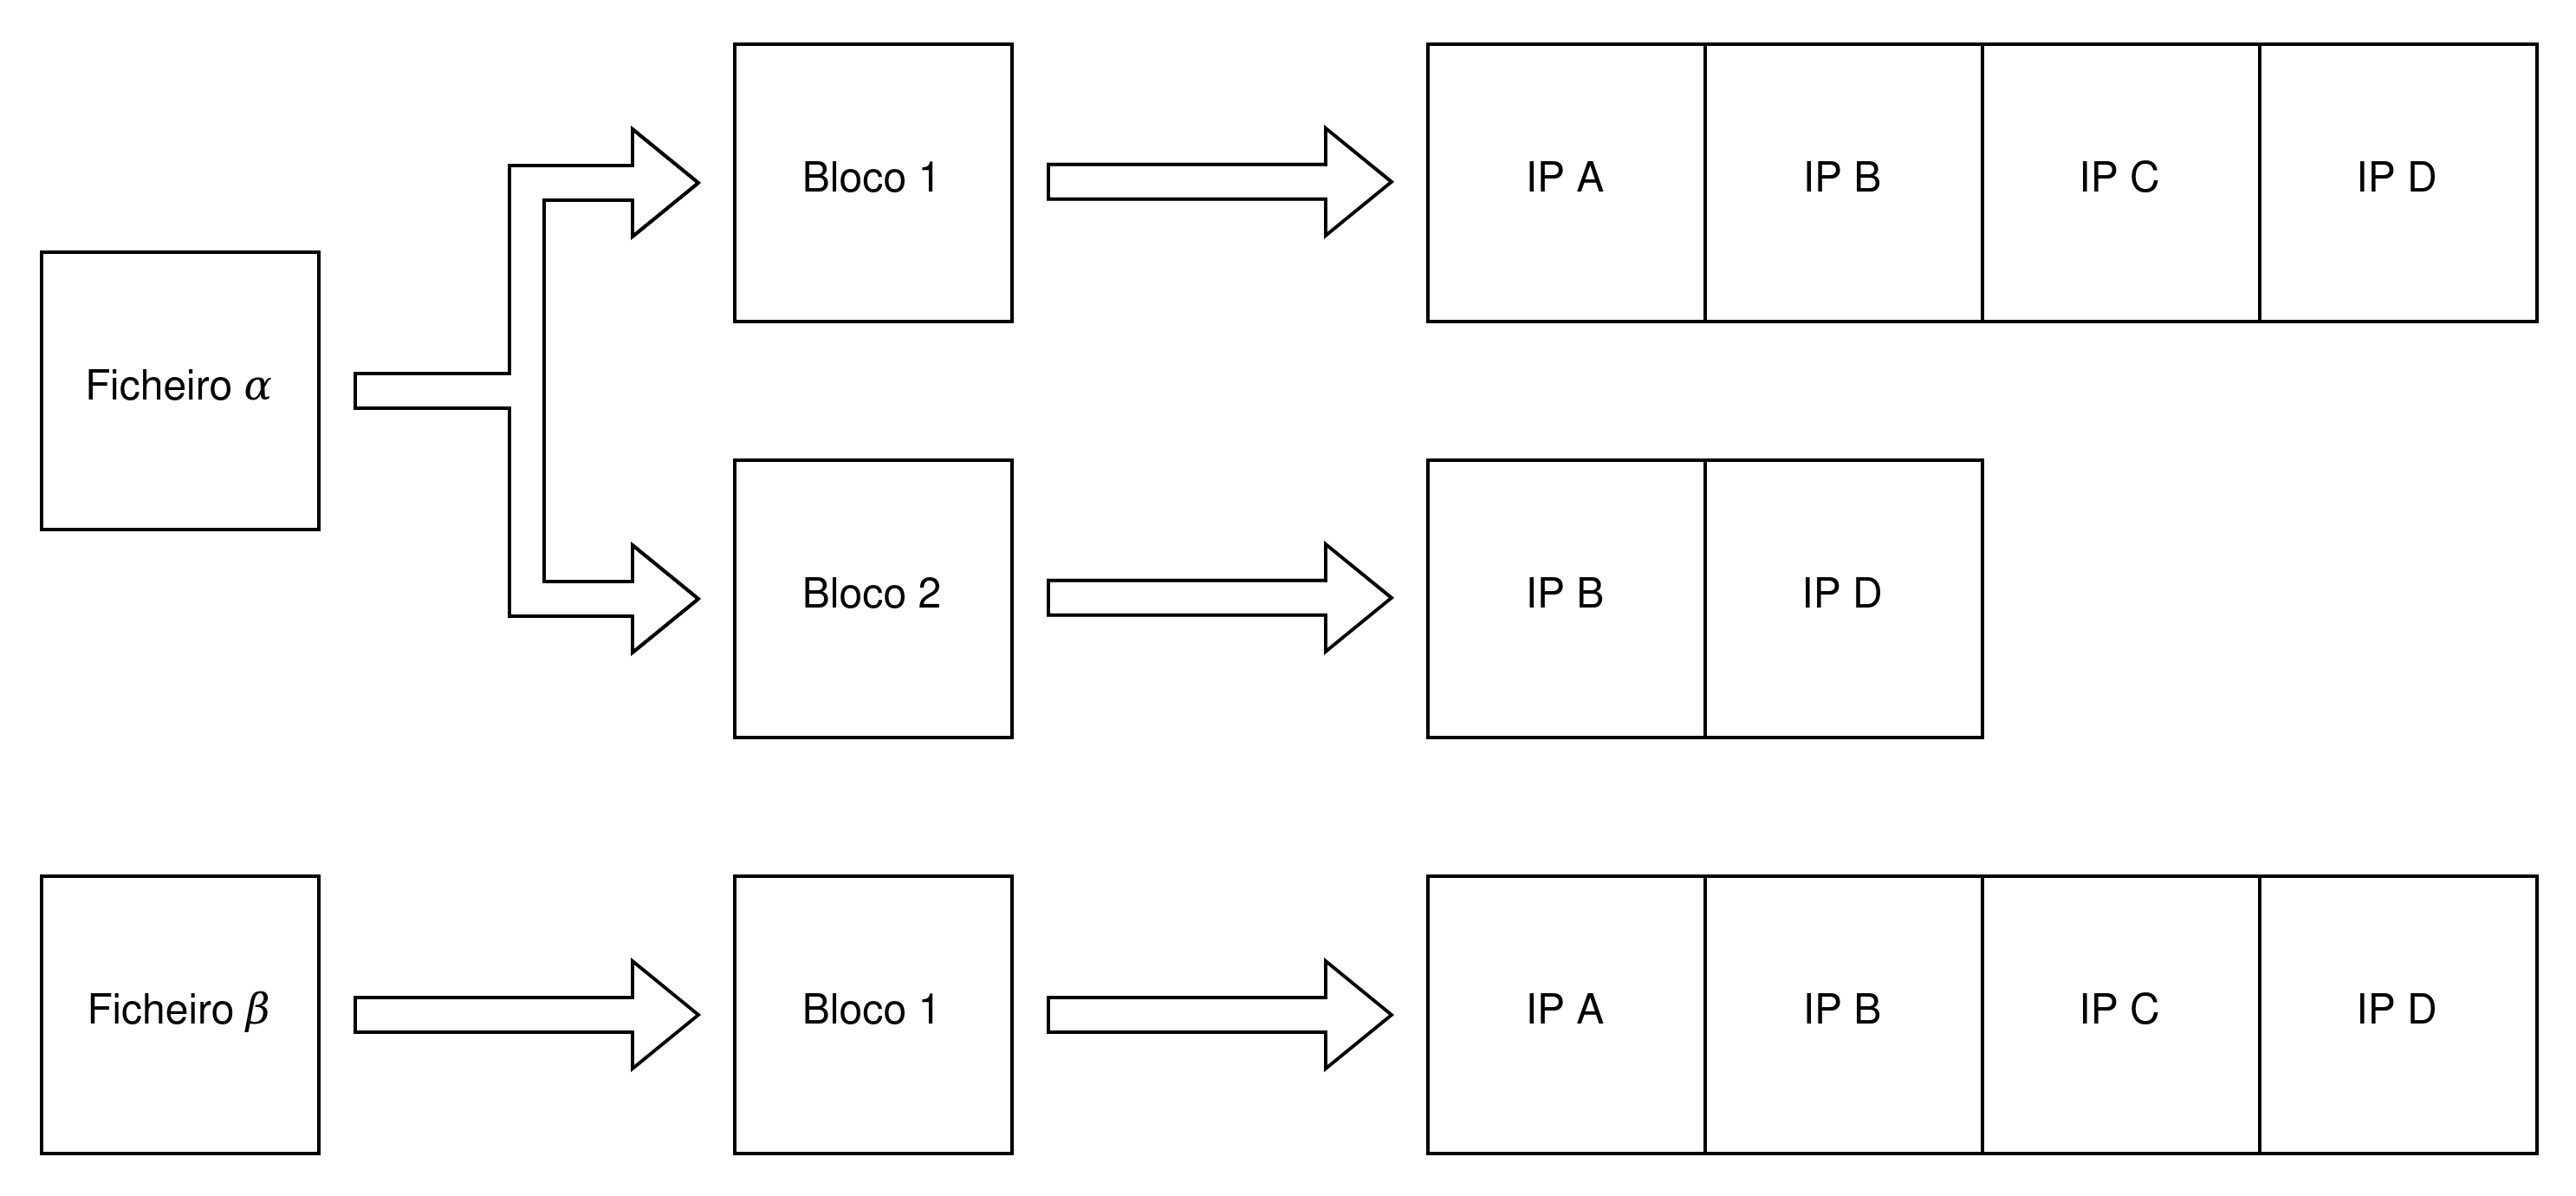
\includegraphics[width=0.85\textwidth]{Imagens/Estruturas/map.png}
            \caption{Esquema da estrutura de dados do \textit{tracker}}
            \label{fig:enter-label}
        \end{figure}
\section{FS Transfer Protocol}

    Depois do \textit{tracker} fornecer todas as informações necessárias à aquisição dos ficheiros pretendidos, o cliente pode iniciar de imediato o processo de transferência com os restantes nós.

    Tal como para o protocolo anterior, também neste caso definimos um segmento capaz de suportar todas as informações necessárias à transferência de ficheiros, o que por sua vez facilita bastante o desenvolvimento de código, no sentido em que apenas uma estrutura de dados é serializada/deserializada.

    Fora isso, e tendo em consideração que os segmentos são enviados a partir de um \textit{datagram socket}, torna-se evidente a necessidade de existirem campos que permitam o controlo de fluxo e erros.

    \newpage
    \begin{figure}[hb!]
        \centering
        \includegraphics[width=0.45\textwidth]{Imagens/Headers/node.png}
        \caption{Cabeçalho de um \textit{UDPPacket}}
    \end{figure}

    O cabeçalho apresentado é bastante semelhante ao de um \textit{TCPPacket}, excetuando os campos \textit{Número de Sequência} (possibilita a ordenação dos blocos) e \textit{Checksum} (permite a identificação de erros).

    A presença dos campos \textit{IP} e \textit{Porta Origem} pode levantar algumas questões, visto que por norma estes seriam facilmente obtidos através de métodos que a própria linguagem de programação disponibiliza, todavia acreditamos que desta forma obtemos uma implementação mais robusta e independente.

    \subsection{Threads}

        Um cliente pode ser contactado a qualquer momento pelos restantes, como tal é necessário atender os pedidos e fornecer as respetivas respostas. Tendo isto em mente, cada cliente possui uma \textit{thread} à escuta numa determinada porta que é conhecida \textit{a priori} por todos os nós da rede.

        Depois de receber e analisar um determinado segmento, o cliente em questão deve assegurar uma resposta, contudo não pode permitir que outros pedidos fiquem por atender, como tal é necessário criar uma nova \textit{thread} cuja função será única e exclusivamente retorquir o pedido em causa.

        A princípio pensámos que seria uma mais-valia criar uma \textit{thread pool}, visto que isso permite a reutilização de \textit{threads}, contudo reparámos que a \textit{thread} principal poderia bloquear caso o tamanho do \textit{buffer} fosse relativamente pequeno quando comparado com a quantidade de nós na rede.

        Ao definirmos que um pedido dá origem a uma \textit{thread}, obtemos um programa significativamente menos eficiente, contudo garantimos que ninguém irá bloquear, seja em que situação for.

        \newpage
        \begin{figure}[hb!]
            \centering
            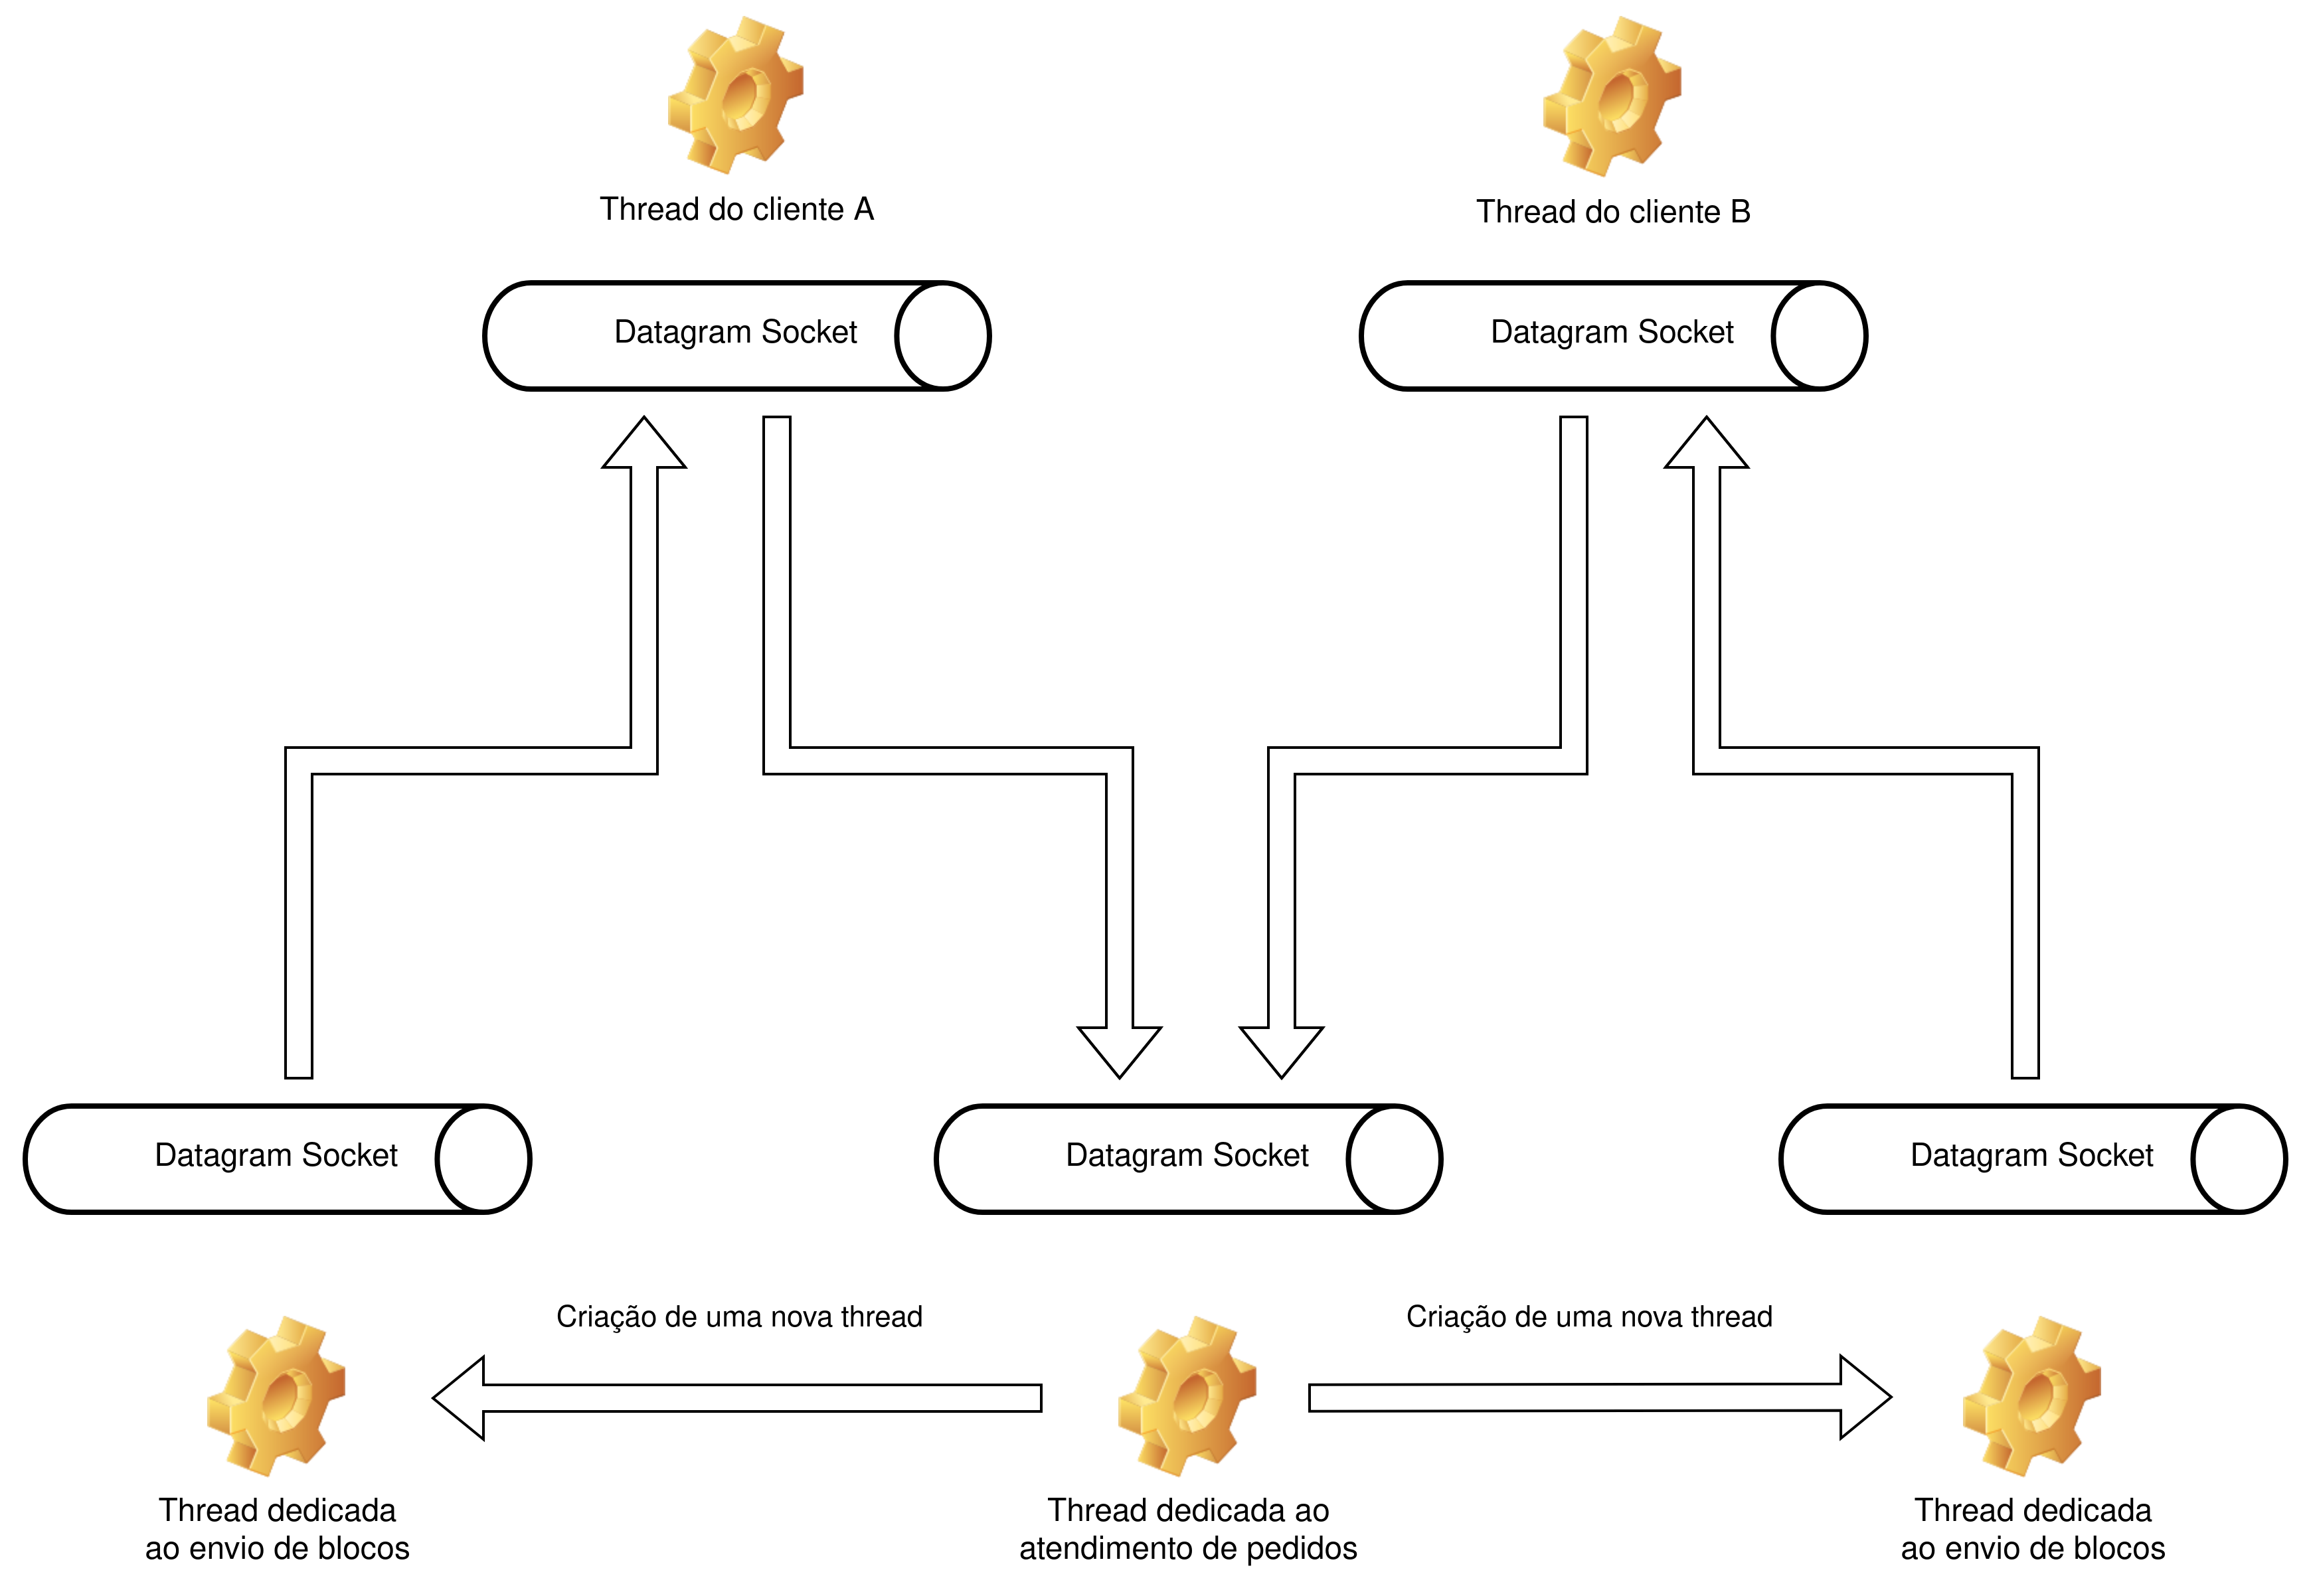
\includegraphics[width=0.75\textwidth]{Imagens/Estruturas/threads.png}
            \caption{Arquitetura do atendimento de pedidos}
        \end{figure}    

    \subsection{Funcionamento}

        Tendo a noção de como os pedidos são atendidos, e conhecendo perfeitamente a estrutura de um \textit{UDPPacket}, podemos especificar o comportamento normal da comunicação entre dois clientes, a fim de um deles obter um determinado conjunto de blocos.

        \begin{enumerate}
            
            \item O cliente \textit{A} envia um \textit{UDPPacket} cujo protocolo corresponde a \textit{HELLO}.

            \item O cliente \textit{B} recebe o segmento e percebe que o \textit{A} quer contactar consigo.

            \item O cliente \textit{B} cria uma \textit{thread} que irá responder ao \textit{A}.

            \item O cliente \textit{B} envia um \textit{UDPPacket} com protocolo \textit{HELLO}, indicando a porta que deverá ser utilizada.

            \item O cliente \textit{A} envia vários \textit{GET's} que contêm os identificadores dos blocos que pretende obter.

            \item O cliente \textit{B} recebe os segmentos e recolhe os blocos pretendidos pelo cliente \textit{A}.

            \item O cliente \textit{B} envia diversos \textit{DATA's} com as informações dos blocos.

            \item O cliente \textit{A} percebe que possui todos os blocos requisitados e escreve-os em disco.

            \item O cliente \textit{A} anuncia ao \textit{tracker} que possui um ficheiro novo.

        \end{enumerate}
        
        \newpage
        \begin{figure}[hb!]
            \centering
            \includegraphics[width=0.75\textwidth]{Imagens/Diagramas Temporais/node.png}
            \caption{Diagrama temporal da comunicação entre clientes}
        \end{figure}

    \subsection{Sliding Window}

        A utilização de \textit{datagram sockets} não assegura que os segmentos enviados cheguem de facto ao seu destino, como tal é necessário estabelecer um pequeno algoritmo que permita isso mesmo, algoritmo esse que se baseia fundamentalmente nos seguintes pontos.

        \begin{itemize}
            
            \item A receção de um segmento é confirmada com o envio de um \textit{acknowledgement}.

            \item A não receção de um \textit{acknowledgement} implica necessariamente que o segmento não chegou corretamente.

            \item Depois de receber todos os \textit{acknowledgements} expectáveis, o emissor aborta o envio de segmentos.

            \item Ao não receber nenhum segmento, o recetor conclui que o emissor já enviou tudo.

            \item O \textit{timeout} do recetor é bastante superior ao do emissor, não permitindo que este seja induzido em erro.
            
        \end{itemize}

        Com estes pontos bem assentes, podemos definir uma versão do algoritmo de \textit{sliding window} utilizado pelo TCP. Ao analisarmos esta estratégia, verificámos que à partida era enviada uma determinada quantidade de segmentos \textit{(window size)}, contudo, a partir daí, havia uma certa tendência para bloqueios, visto ser necessário receber o \textit{acknowledgement} do elemento que estava na primeira posição da janela.

        Esta situação parece-nos um pouco estranha e desnecessária, portanto a nossa versão do \textit{sliding window} procura corrigir essa tendência para bloqueios.

        \begin{wrapfigure}{r}{0.4\textwidth}
            \begin{center}
            \vspace{-25pt}
            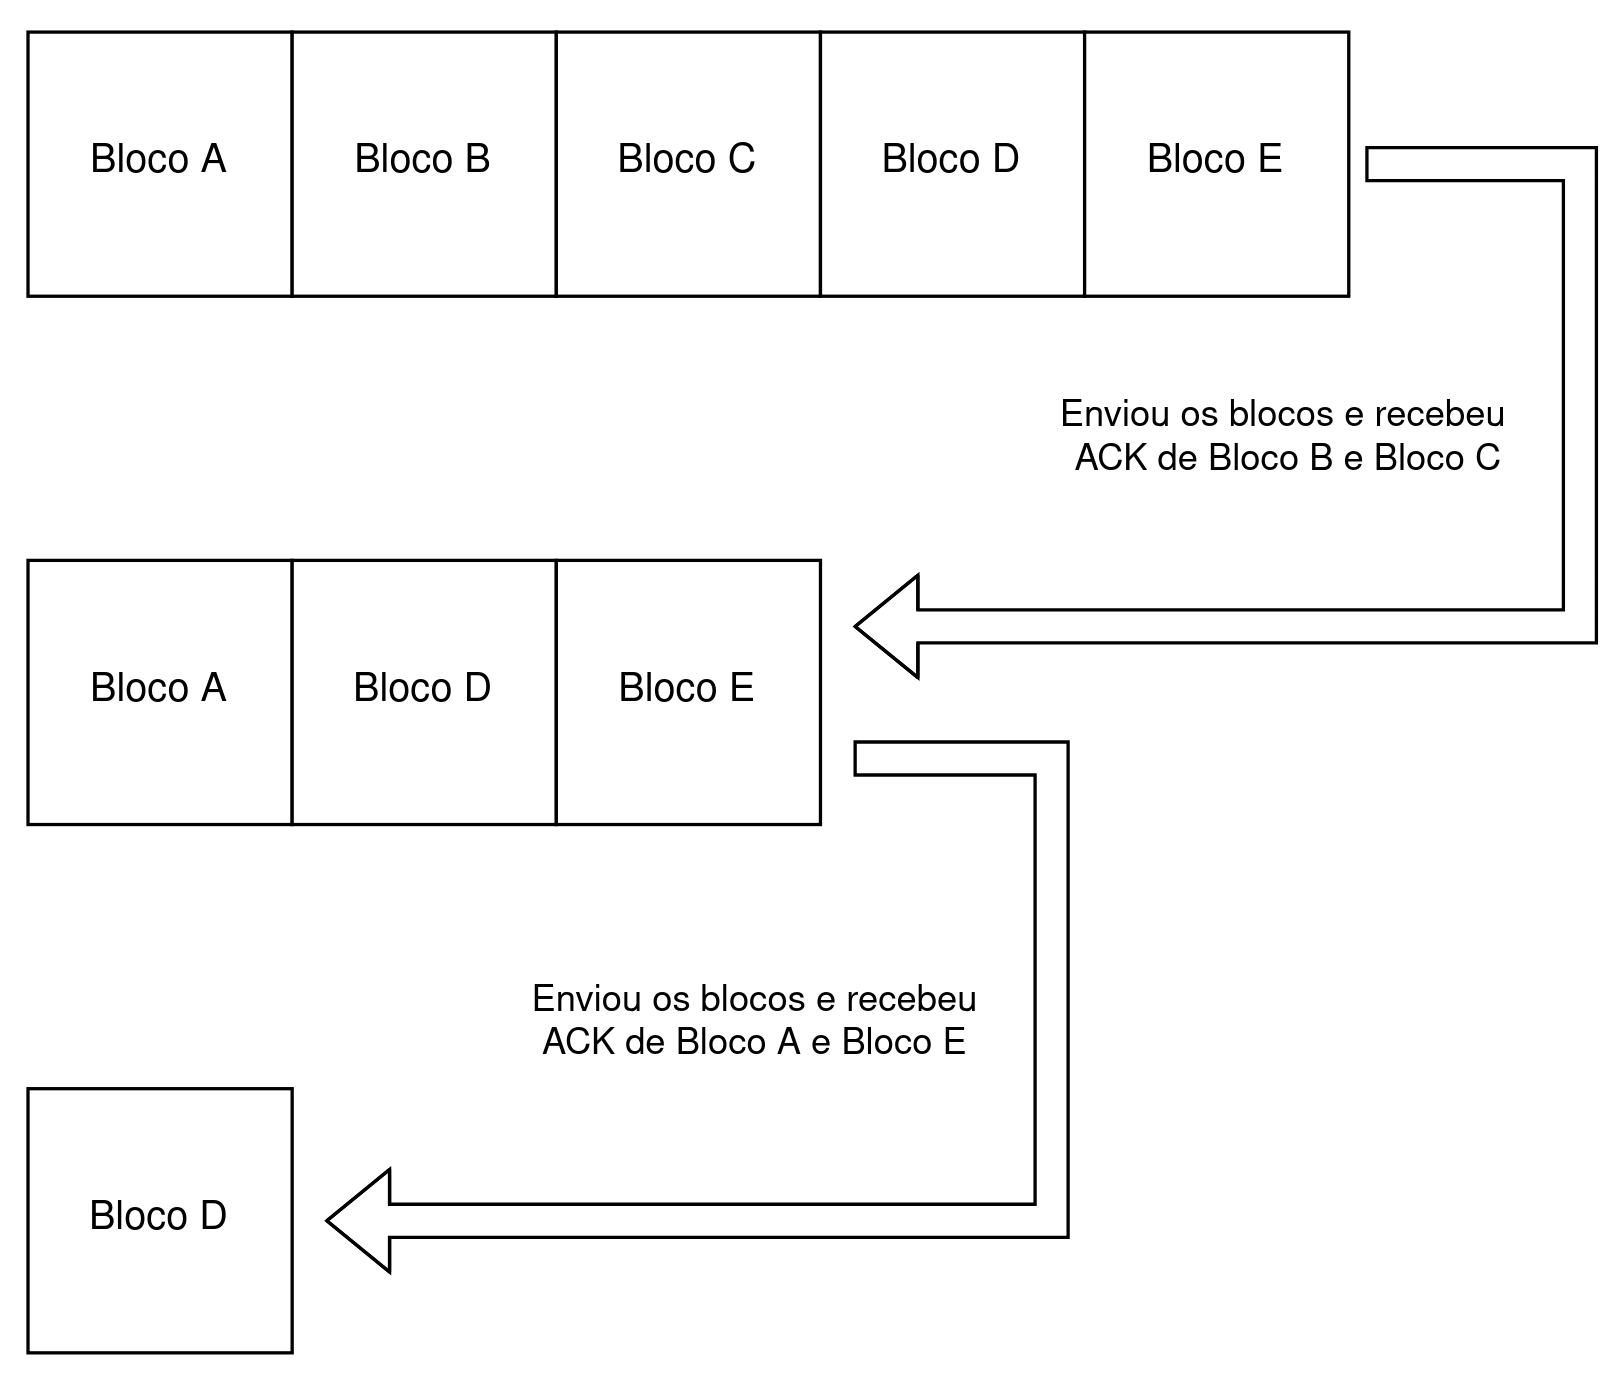
\includegraphics[width=0.4\textwidth]{Imagens/Estruturas/node blocos.png}
            \caption{\textit{Buffer} de blocos}
            \vspace{-50pt}
            \end{center}
        \end{wrapfigure}

        \hspace{4.5pt}1.~ O emissor define um \textit{timeout} bastante inferior ao do recetor.

        \hspace{4.5pt}2.~ O emissor criar um \textit{buffer} onde constam os segmentos.
            
        \hspace{4.5pt}3.~ O emissor envia uma determinada quantidade de segmentos.
        
        \hspace{4.5pt}4.~ O emissor aguarda a chegada de um \textit{acknowledgement}.

        \hspace{4.5pt}5.~ A receção de uma confirmação apaga um segmento do \textit{buffer.}

        \hspace{4.5pt}6.~ O emissor envia outro segmento e repete os passos 4 e 5.

        \hspace{4.5pt}7.~ Depois de enviar o último segmento, volta ao início.

        \hspace{4.5pt}8.~ O processo termina quando todas as confirmações chegarem.

        \begin{wrapfigure}{r}{0.4\textwidth}
            \begin{center}
                \vspace{-25pt}
                \includegraphics[width=0.35\textwidth]{Imagens/Diagramas Temporais/udp.png}
                \caption{Diagrama temporal}
                \vspace{-50pt}
            \end{center}
        \end{wrapfigure}

        Ao analisarmos o diagrama temporal correspondente ao envio de segmentos, percebemos claramente a vantagem desta reformulação do algoritmo de \textit{sliding window}.

        Supondo uma janela de tamanho dois, originalmente o algoritmo começa por enviar dois segmentos \textit{(A e B)}, todavia, para poder prosseguir, é necessário que chegue o \textit{acknowledgement} do segmento \textit{A}, algo que não acontece.

        Posto isto, a janela iria ficar bloqueada até que o \textit{acknowledgement} desejado chegasse, o que não é minimamente aconselhável se queremos tirar o máximo partido da rede.

        Assim sendo, na nossa implementação, a janela continua a deslizar sem se preocupar que os segmentos tenham sido corretamente enviados, visto que após chegar ao fim do \textit{buffer}, o processo irá repetir-se de modo a que os segmentos não confirmados sejam retransmitidos.

        Apesar de promissora, esta solução acaba por criar um novo problema capaz de saturar qualquer rede num instante. Embora um segmento tenha chegado corretamente ao seu destino, o mesmo será retransmitido várias vezes, pois o \textit{timeout} do emissor é demasiado curto, o que origina imensas replicações de dados.

    \subsection{Controlo de Erros}

        A utilização de \textit{datagram sockets} não garante vários aspetos, entre eles a integridade dos segmentos, como tal é necessário definir uma estratégia que permita ao recetor perceber se uma dada mensagem foi corrompida.

        A princípio pensámos em utilizar \textit{SHA-1}, todavia percebemos que essa função de \textit{hash} não era apropriada para efetuar controlo de erros, sendo um dos motivos apontados a complexidade que o algoritmo exige.

        Desta forma, é fundamental procurar um balanço entre a eficácia na detenção de erros, e a complexidade na criação do \textit{hash}, assim sendo, chegámos a um algoritmo designado de \textit{CRC32C}, que pelos vistos é o sucessor do \textit{CRC32} utilizado pelo \textit{layer 2}.

        Após efetuarmos a transferência de milhões de segmentos entre nós do \textit{CORE}, verificámos que o nosso algoritmo de deteção de erros não foi ativado uma única vez, o que nos levou a formular algumas hipóteses.

        \begin{itemize}
            
            \item Será que o controlo de erros efetuado pelas camadas inferiores foi tão eficaz ao ponto de não detetarmos qualquer erro no nível aplicacional?

            \item Será que a linguagem de programação utilizada garante a integridade dos dados caso eles cheguem ao seu destino?

        \end{itemize}

        A primeira hipótese não tem grande credibilidade, portanto fomos ler de imediato a documentação do \textit{Java}, e tendo em conta que este tema não estava mencionada nos avisos sobre a utilização de \textit{datagram sockets}, a segunda hipótese é afinal verdadeira, pelo que o controlo de erros é realizado implicitamente.
\section{Domain Name System}

    A utilização de um sistema de resolução de nomes permite que o \textit{tracker} conheça o nome dos \textit{end systems} em vez dos seus endereços IP, como tal é essencial realizar algumas alterações no segmento \textit{TCPPacket}, nomeadamente acrescentar um campo \textit{hostname}.

    Durante as aulas práticas foi mencionado que deveríamos usufruir de uma solução que tivesse por base \textit{bind}, algo que estudamos durante imenso tempo e tentámos implementar.

    Infelizmente desistimos desse caminho, pois nenhum docente forneceu-nos qualquer base sobre como utilizar o serviço \textit{bind9} na topologia do \textit{CORE}, e quando descobrimos já era tarde de mais para poder voltar atrás.

    Assim sendo, fomos obrigados a implementar um protocolo de DNS e o seu respetivo servidor, percebemos que seria importante haver uma redundância de servidores DNS, contudo o tempo urge e não nos permite qualquer margem de manobra.

    Em termos práticos, um servidor DNS possui um \textit{map} no qual associa \textit{hostnames} a endereços IP, como tal o cabeçalho dos segmentos utilizados para resolver um determinado nome é bastante simplista.

    \newpage
    \begin{figure}[hb!]
        \centering
        \includegraphics[width=0.45\textwidth]{Imagens/Headers/dns.png}
        \caption{Cabeçalho de um \textit{DNSPacket}}
    \end{figure}

    O campo \textit{Protocolo} pode parecer um pouco inútil, visto que o único objetivo deste serviço é resolver um determinado nome, todavia torna-se crucial nos momentos em que é necessário avisar o servidor DNS do aparecimento/desaparecimentos de nós.

    Originalmente o DNS usufrui do UDP como forma de maximizar a velocidade do serviço, todavia optámos por utilizar TCP, visto que isso facilita bastante a implementação do código.

    \begin{figure}
        \centering
        \includegraphics[width=0.47\textwidth]{Imagens/Diagramas Temporais/dns.png}
        \caption{Diagrama temporal da resolução de nomes}
    \end{figure}

    \begin{enumerate}
        
        \item O cliente pretende obter o endereço IP associado a um \textit{hostname}.

        \item É enviado um \textit{REQUEST} ao servidor DNS.

        \item O servidor DNS verifica se o \textit{hostname} recebido existe na sua estrutura de dados.

        \item Em caso afirmativo é envidado um \textit{RESPONSE} com o endereço IP, caso contrário é transmitido um \textit{ERROR}.

    \end{enumerate}
\section{Conclusão}

    Ao longo da realização deste trabalho prático enfrentámos vários desafios que nos obrigaram a pensar com espírito crítico e a refletir sobre quais seriam as melhores estratégias a adotar em cada situação, nomeadamente na definição de cabeçalhos e na arquitetura dos \textit{end systems}.

    Voltando atrás e analisando todo o caminho percorrido, pensamos que teria sido uma mais-valia aplicar \textit{bind9} no projeto, visto que isso tornaria o sistema relativamente mais robusto e flexível. Assim sendo, no futuro, desejamos vir a explorar mais detalhadamente este serviço, pois claramente muitos pontos ficaram por esclarecer. 

    Em suma, e apesar dalguns contratempos, julgámos que este trabalho prático foi útil no sentido em que consolidou alguns conceitos que tinham ficado pouco claros nas aulas teóricas, e além disso, abriu-nos os olhos para a complexidade exigida no nível aplicacional quando se utiliza o UDP enquanto protocolo da camada transporte.

\end{document}